\pagebreak
\section{Edges and Gradients}
\subsection{Overall rationale and theory}
Extending on the previously described means of detecting the pupil, image
intensity gradients provide a method for finding the edge between pupil and
iris, as well as the limbus (the edge between iris and sclera). The problem of
finding edges in an image can be reduced to the problem of finding high
magnitudes in the image's gradients.
In practice:
\begin{itemize}
	\item Noise reduction is performed,
	\item The image gradients are found, and
	\item A subset of the gradients are scanned to determine the location of edges in the
original image.
\end{itemize}

\begin{figure}[htbp]
%\centering
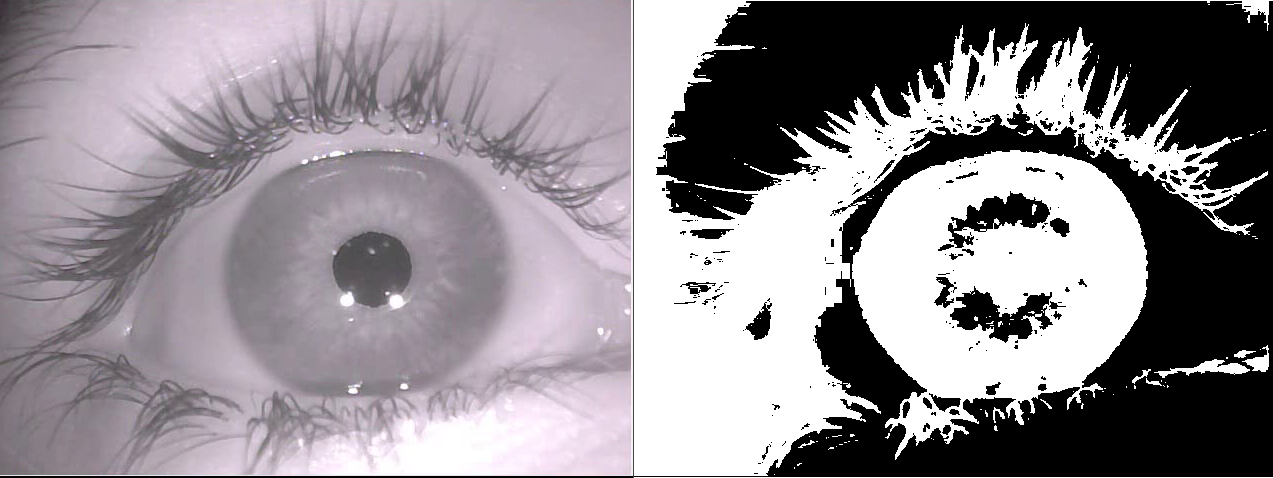
\includegraphics{pics/iris_threshold.png}
\caption{An attempt at using binary thresholding to locate the iris.
while the iris is not a continuous blob, it is starting to converge with the sclera.}
\label{fig:iristhresh}
\end{figure}

This solution is explored partly as an alternative to finding the limbus via
thresholding. Figure \ref{fig:iristhresh}, illustrates the difficulty of finding a good threshold for the iris. 


\begin{figure}[htbp]
%\centering
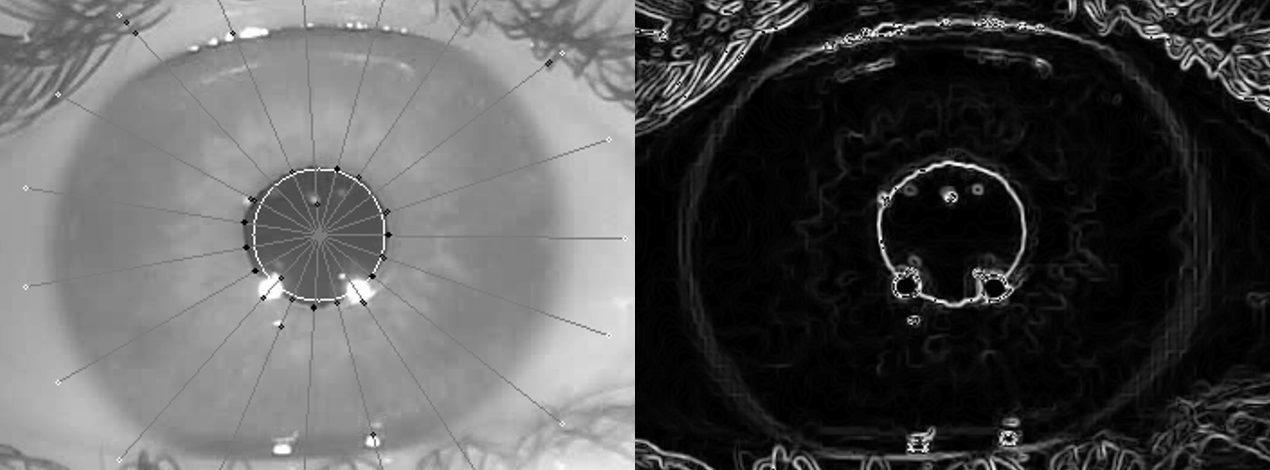
\includegraphics{pics/normallines_with_maxima_vs_gradient.png}
\caption{\textbf{Left:} Black dots are the highest gradient magnitudes found on the grey
lines (here, 2 per line). The white circle is the initial estimate of the
pupils location. \textbf{Right:} The set of gradient magnitudes represented as an image.}
\label{fig:normalsVsGradient}
\end{figure}

\subsection{Using gradient magnitudes}
A bilateral filter was chosen for noise reduction. In contrast to blurs like
Gaussian filters, bilateral filters weigh the inputs according to both
euclidean distance to the output pixel, and the intensities in the source
patch. The consideration of intensity differences makes bilateral filters edge
preserving which, not surprisingly, is crucial for edge detection.

The image gradients are found by applying the sobel operator on the image. In
effect; finding approximated partial derivatives for the vertical and
horizontal axes respectively. Together, the two derived images form a set of
vectors, each describing the gradient for its pixel location. The length of one
of these vectors is the gradient magnitude of a certain point in the original
image. That is; the rate of change in intensity in a specific pixel. An
''edge'' is a continuous path of high gradient magnitudes. The gradient
magnitude in the point $(i,j)$ is found by $$\sqrt{x^2+y^2}$$ where $$x =
\frac{\delta z}{\delta i}, \quad y = \frac{\delta z}{\delta j}$$ and $z$
denotes pixel intensity. 

The scanned lines are chosen as the normals of a
previously found estimate of pupil, here scaled to 4.5 times the estimate’s
radius, and spaced with 0.314 radians. In principle this method should provide
20 points on the periphery of the pupil, and should be extensible to finding
the limbus. In practice, however, a few problems might arise.

\subsection{Using gradient orientation}
When examining figure \ref{fig:normalsVsGradient}, it becomes obvious that the
pupils edge might not be have the highest gradient magnitude. For example, the
eyelashes and glints might give a larger intensity change, than the
black-to-grey change between pupil and iris.Luckily this problem can be
bettered using information already available, namely the image gradients’
orientations. By considering the gradients angle to the pupil normal, some of
the high gradients can be discarded. This works on the assumption that the
pupil is fairly circular, and that estimated pupil location is somewhat
correct. Thus, the angle between normal and gradient on the pupil edge will be
small.The gradients’ angles to the positive x-axis is found and compared to the
normals angle to the positive x-axis. The angle between a vector and the
positive x-axis can be found by applying the arctangens2 operator to its
lengths: atan2$(x,y)$.

The use of gradient orientation presents a new problem; performance. The use of
the atan2 operator proves to be heavy enough that it became necessary to reduce
the size of the input image. As this method assumes a previous estimate of the
pupil’s location, it might be preferable to select an image patch around the
eye, rather than actually down sampling the input image. Though the latter will
be less robust to change in eye size or distance to the camera.

The described method is applicable to limbus detection, but in practice the
iris is much harder to detect. This is probably due to the smaller contrast
between iris and sclera, as well as to the edge between them being ‘jagged’
(this is most visible in the right side of iris in the above gradient image).
